\documentclass[12pt]{article}

%to add an affiliation line to the the title formatting
\usepackage{authblk}

%Fonts
\usepackage[no-math]{fontspec} %This allows you to enter (via an IPA kayboard) IPA fonts and other symbols directly into LaTeX. Requires a particular setyp, see below.
\usepackage{libertine} %A font that actually contains many IPA symbols. This is the font you see in the preview to the right.

%to use these fonts, be sure that your typesetting engine is set to "XeLaTeX." In Overleaf, go to the Menu link on the top left (by the Overleaf icon), and under Settings be sure that the Compiler is set to "XeLaTeX." If you accessed this document via the Overleaf Pomona Linguistics template, all of this was already done for you.

%The Pomona Linguistics Paper Template in Overleaf is already set up for this, but you may run into this problem if you start building your own documents.


%%%%%%%%%%%%%%%%%%%%%%%%%%%%%%%%%%%%%%%%%%%%%%%%%%%
%packages for this style of handout-formatting of (sub)section headers
\usepackage[explicit]{titlesec}
\usepackage{xcolor}

\definecolor{light-gray}{gray}{0.7}
\definecolor{lighter-gray}{gray}{0.85}

\titleformat{\section}
{\normalfont\Large\bfseries}{}{0em}{\colorbox{black}{\parbox{\dimexpr\textwidth-2\fboxsep\relax}{\textcolor{white}{\thesection\quad#1}}}}

\titleformat{\subsection}
{\normalfont\large\bfseries\scshape}{}{0em}{\colorbox{light-gray}{\parbox{\dimexpr\textwidth-2\fboxsep\relax}{\textcolor{black}{\thesubsection\quad#1}}}}

\titleformat{\subsubsection}
{\normalfont\bfseries}{}{0em}{\colorbox{lighter-gray}{\parbox{\dimexpr\textwidth-2\fboxsep\relax}{\textcolor{black}{\thesubsubsection\quad#1}}}}
%%%%%%%%%%%%%%%%%%%%%%%%%%%%%%%%%%%%%%%%%%%%%%%%%%%

%%% This file is the preamble for the Pomona Linguistics LaTeX Paper Template, which is also used for the Quick Reference Guide. If you are brand new to writing with LaTeX, we suggest NOT messing with it, and just writing your paper using the Paper Template. If you are getting more comfortable in LaTeX and want to add packages and commands, this is where you do it (when using this template).

%For stacking text, used here in autosegmental diagrams
\usepackage{stackengine}

%To combine rows in tables
\usepackage{multirow}

%geometry helps manage margins, among other things.
\usepackage[margin=1in]{geometry}

%Gives some extra formatting options, e.g. underlining/strikeout
\usepackage{ulem}

%For putting links into papers, also helps make cross-references in the paper smart references
\usepackage[colorlinks = true,
            linkcolor = blue,
            urlcolor  = blue,
            citecolor = blue,
            anchorcolor = blue]{hyperref} %smarter cross-references, these options turn links blue

%Use package/command below to create a double-spaced document, if you want one. Uncomment BOTH the package and the command (\doublespacing) to create a doublespaced document, or leave them as is to have a single-spaced document.
%\usepackage{setspace}
%\doublespacing

%paragraph formatting
\usepackage[parfill]{parskip}
\setlength{\parskip}{5pt} %plus 1 minus 1}
\setlength{\parindent}{30pt}
\usepackage{titlesec}

%use for special OT tableaux symbols like bomb and sad face. must be loaded early on because it doesn't play well with some other packages
\usepackage{fourier-orns}

%Basic math symbols
\usepackage{pifont}
\usepackage{amssymb}

%%%Gives shortcuts for glossing. The use of this package is NOT explained in the Quick Reference Guide, but the documentation is on CTAN for those that are interested. MJKD finds it handy for glossing. (https://ctan.org/pkg/leipzig?lang=en)
\usepackage{leipzig}

%Tables
\usepackage{caption} %For table captions
\usepackage{booktabs} %helps format tables

%For citations and bibliography - as of 9.1.2019 we don't explain citations in this Quick Reference Guide, but Pedro Martin's tutorial does (see links in the Guide).
\usepackage{natbib}

%For OT-style tableaux
\usepackage{ot-tableau}

%highlights text with \hl{text}
\usepackage{color, soul}

%Drawing Syntax Trees
\usepackage[linguistics]{forest}

%This specifies some formatting for the forest trees to make them nicer to look at
\forestset{
  nice nodes/.style={
    for tree={
      inner sep=0pt,
      fit=band,
    },
  },
  default preamble=nice nodes,
}

%% For numbered and glossed examples %%
\usepackage{gb4e}



%Changes the \maketitle command to be smaller and take up less space on a page.
\makeatletter
\def\@maketitle{   % custom maketitle
\noindent {\Large \bfseries \color{black} \@title}  \\ \hrule \noindent \@author \\ \@date
}

%The code below will draw a circle around a piece of text. This is very useful for drawing attention to a word in a data example. use the command \circled{text} where the argument (`text' here) is what you want to be circled. This is illustrated in the Quick Reference Guide and the Paper Template.

\usepackage{tikz}

\newcommand{\circled}[1]{\begin{tikzpicture}[baseline=(word.base)]
\node[draw, rounded corners, text height=8pt, text depth=2pt, inner sep=2pt, outer sep=0pt, use as bounding box] (word) {#1};
\end{tikzpicture}
}


%%%%%%%%%%%%%%%%%%%%%%%%%%%%%%%%%%%%%%%%%%%%%%%%%%%%%%%%%%%%
%%%%%%%%%%%%%%%%%%%%%%%%%%%%%%%%%%%%%%%%%%%%%%%%%%%%%%%%%%%%

% Useful Ling Shortcuts

\RequirePackage{leipzig}
%\RequirePackage{mathtools} % for \mathrlap

% % % Shortcuts  (borrowed from JZ, I'm still unsure exactly what xspace requires)
\RequirePackage{xspace}
\xspaceaddexceptions{]\}}

%This makes the \emptyset command be a nicer one
\let\oldemptyset\emptyset
\let\emptyset\varnothing
\newcommand{\nothing}{$\emptyset$}

%Not all of these are explained in the Quick Reference Guide, but they are here bc they are relevant to some of our students.
\newcommand{\1}{\rlap{$'$}\xspace}
\newcommand{\0}{\rlap{\textsuperscript{$ˆ{\circ}$}}\xspace}
\newcommand{\Lb}[1]{$\text{[}_{\text{#1}}$ } %A more convenient left bracket
\newcommand{\Rb}[1]{$\text{]}_{\text{#1}}$ } %A more convenient left bracket
\newcommand{\gap}{\underline{\hspace{1.2em}}}
\newcommand{\vP}{\emph{v}P}
\newcommand{\lilv}{\emph{v}}
\newcommand{\Abar}{A$'$-} %A more convenient A-bar notation
\newcommand{\ph}{$\varphi$\xspace} %A more convenient phi
\newcommand{\pro}{\emph{pro}\xspace}
\newcommand{\subs}[1]{\textsubscript{#1}} %A more convenient subscript
%\newcommand{\hd}{$^{\circ}$\xspace} %Symbol for printing head / degree symbol
\newcommand{\spells}{$\Longleftrightarrow$} %spellout arrow for morph spellout rules
\newcommand{\tr}[1]{\textit{t}\textsubscript{\textit{#1}}} %easy traces with subscript
\newcommand{\supers}[1]{\textsuperscript{#1}}

% Abbreviations for glossing, based on Leipzig
\newleipzig{hab}{hab}{habitual}
\newleipzig{rem}{rem}{remote}
\newleipzig{sm}{sm}{subject marker}
\newleipzig{t}{t}{tense}
\newleipzig{aa}{aa}{anti-agreement}
\newleipzig{pron}{pron}{pronoun}
\newleipzig{rec}{rec}{recent}
\newleipzig{om}{om}{object marker}
%\newleipzig{ipfv}{ipfv}{imperfective}
\newleipzig{asp}{asp}{aspect}
\newleipzig{lk}{lk}{linker}
\newleipzig{pcl}{pcl}{particle}
\newleipzig{stat}{stat}{stative}
\newleipzig{ints}{ints}{intensive}
\newleipzig{ascl}{ascl}{assertive subject clitic}
\newleipzig{nascl}{nascl}{non-assertive subject clitic}
\newleipzig{ta}{ta}{tense and/or aspect}
\newleipzig{assoc}{assoc}{associative marker}
\newleipzig{hon}{hon}{honorific}
%\newleipzig{whprt}{wh}{\wh particle}
\newleipzig{sa}{sa}{subject agreement}
\newleipzig{conj}{conj}{conjunction}
%\newleipzig{loc}{loc}{locative}
\newleipzig{expl}{expl}{expletive}
\newleipzig{rcm}{rcm}{reciprocal marker}
\newleipzig{pers}{pers}{persistive}
%\newleipzig{}{}{} %this is just to copy for when I want to add more

%%%%%%%%%%%%%%%%%%%%%%%%%%%%%%%%%%%%%%%%%%%%%%%%%%%%%%%%%%%%
%%%%%%%%%%%%%%%%%%%%%%%%%%%%%%%%%%%%%%%%%%%%%%%%%%%%%%%%%%%%

%A couple of packages that seemed to prefer being called toward the end of the preamble

%This package provides macros for typesetting SPE-style phonological rules.
\usepackage{phonrule}

%For using Greek letters outside of math mode.
%\usepackage{textgreek}


%Random, lets us use the XeLaTeX logo. Not important to the template at all.
\usepackage{metalogo}


%%%%%%%%%%%%
%% This is the end of the PREAMBLE
%%%%%%%%%%%


\title{Introduction to Tariana}
\author{Skylar Litz}
\date{February 17, 2021}

\begin{document}

\maketitle

%\textbf{Goals of talk:} This is a handout including (mainly) word order of clauses and noun phrases, as well as other major features necessary to understand the basics of the language (e.g. basic morphology on nouns and verbs).

\section{Introduction}
 Tariana is an Arawak language spoken in the multilingual area of the Vaupés basin in northwestern Brazil. All data, examples, and generalizations presented here come from Aikhenvald (2003).
\section{Constituent Order}
  Tariana is a \textbf{`pragmatically ordered'} language so establishing a basic constituent order is not possible. In both texts and conversations, any constituent order is possible and all different organizations are used.

\subsection{Details on Pragmatic Ordering}
\begin{itemize}
  \item Sentences that are translated from the nearby language Tucano are generally \textit{verb-final} while sentences translated from Portuguese are often \textit{verb-medial}. For this reason, when studying Tariana it is important not to rely on translated material to understand constituent order.

  % pg 586 of pdf
  \item Instead of having a set constituent order, pragmatic parameters are used to order constituents in main clauses. These parameters include new vs. old information, relative topicality, definiteness, specificity, and contrast.

  \item There are also specific case markings for topicality of a non-subject constituent, specific and/or definite referents, and focussed and contrastive subjects.

  % go over these in next presentation?
  %\item Clause initial and pre-predicate positions: Topicality
  %\item Post-predicate positions: contrast and/or disambiguation
  %\item Unmarked non-subject immediately before the predicate

  % pdf pg 591
  \item There are a few constructions that maintain a fixed constituent order. These are,
  \begin{itemize}
    \item position of the copula component with respect to the copula
    \item position of interrogative words
    \item position of clause connectors
    \item position of the predicate in dependent clauses
    \item imperatives and apprehensives
    \item double S-clauses
  \end{itemize}

  \item A unique feature of Tariana compared to other Arawak languages is that in possessive constructions, the possessor always precedes the possessed noun.

\end{itemize}


\section{Order of words in Noun Phrases}
A noun phrase consists of a head plus one or more modifiers.

  \subsection{NP heads}
  \begin{itemize}
    \item NP heads can be a noun, adjective, or a member of certain closed classes (demonstratives, specifier articles, quantifier, and deictics).
    \item The head of an NP forces classifier (or animacy) agreement on any modifier that is present on the head. %[SEE CHAPTER 5] (more on this in second presentation? or add diarrhea example from page 93 (pdf pg 116))
    %\item If the NP head is animate, number agreement is also required (see 8.4)
  \end{itemize}
  \subsection{NP modifiers}
  \begin{itemize}
    \item Modifiers can be adjectives, members of certain closed classes, and some nouns.
    \item Adjectives or closed class modifiers can be used in either the prehead or posthead position, except for specifier articles, demonstratives, and the quantifier \textit{kanapada} which must always precede the NP head.
    \item The placement of modifiers prehead or posthead depends on the definiteness and specificity of the head noun. If a noun is definite or specific, modifiers tend to be placed before the noun. Indefinite or non-specific nouns usually have modifiers placed after the noun.
  \end{itemize}
  %\subsubsection{Example}
  For example (Figure \ref*{naughtytapir}), in a story being told about a well-known naughty tapir who destroys gardens, the modifier adjective `bad' is placed before the head noun, `tapir.'

\begin{figure}[h]
  \centering
  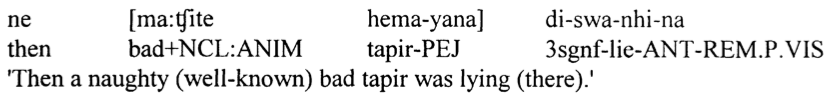
\includegraphics[scale = 0.5]{naughtytapir.png}
    \caption{(Aikhenvald 2003 page 476)}
    \label{naughtytapir}
\end{figure}

  \begin{itemize}
    \item An NP can contain only one prehead modifier, so if one modifier is required to appear before the noun, the rest will appear after.
    % pg 505
    \item In narratives and conversations, full NPs are not very frequent. Instead, headless NPs are used in which a classifier is used to identify the referent.
    %\item possessive constructions the possessor always precedes the possessed noun (different from different Arawak languages) pg 506
  \end{itemize}
For example (Figure \ref*{oneman}), the man who lives alone with his children is introduced in a headless NP with a numeral and a classifier.

\begin{figure}[h]
  \centering
  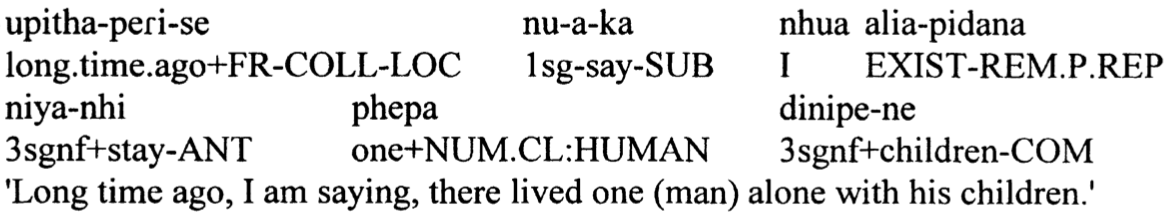
\includegraphics[scale = 0.69]{oneman.png}
    \caption{(Aikhenvald 2003 page 482)}
    \label{oneman}
\end{figure}

\end{document}
